\documentclass{article}

%%%%%%%%PACKAGES%%%%%%%%
\usepackage{amsmath} 
\usepackage{mathtools}
\usepackage{amsfonts}
\usepackage{siunitx} 
\usepackage{physics}
\usepackage{geometry}
\usepackage{graphicx}
\usepackage{float}
\usepackage{hyperref}
\usepackage{url}
\geometry{margin=1in} 

%%%%%%%%TITLE%%%%%%%%
\title{Notes on Chern-Simons Theory}
\author{Gabriel C. Magalhães\footnote{gabriel.capelini@uel.br}}
\date{2026}

\begin{document}
\maketitle

\begin{abstract}
	These notes present  my current understanding of Chern-Simons theory and are intended for pedagogical purposes. They are continuously updated as I learn more about the subject and are based on the references listed in references section.
\end{abstract}

\tableofcontents
\pagebreak

\section{Introduction}
 In this note, we will start by studying one of the simplest, but richest, theory with topological degrees of freedom. This is called \textit{Chern-Simons theory}. Chern Simons theory is of great importance because it is the Effective Field Theory (EFT) for the Quantum Hall Effect (QHE). Before we proceed, we briefly introduce QHE to motivate some later discussions. Here we follow the discussions of \cite{dunne_aspects_1999,tong_lectures_2016}.
\section{Quantum Hall Effect}
The Quantum Hall Effect (QHE) is a remarkable physical phenomenon that arises under extreme conditions, low temperatures and strong magnetic fields, where the Hall conductance becomes quantized. The QHE’s deep connection to topology is revealed through its effective field theory description, which is a gauge theory in (2+1) dimensions called the \textit{Chern-Simons Theory,} which, as we will see, depends only on the underlying topology of the theory. The Chern-Simons theory is the first theory that we will study that has topological degrees of freedom. In this section, we give a brief overview on the QHE to motivate some physical arguments that we will use when talking about Chern-Simons theory. For a more detailed description, see \cite{tong_lectures_2016}.
\subsection{Classical Hall Effect}
The Hall Effect consists in a plane with a current $I$ (let us suppose that it lies in the $x$-direction), and magnetic field $\vec{B}$ applied in the $z$-direction. The magnetic field bends the current towards the $y$-direction, which produces a potential difference $V_H$, where $H$ stands for Hall. The Scheme can be seen in the figure below 
\begin{figure}[H]
	\centering
	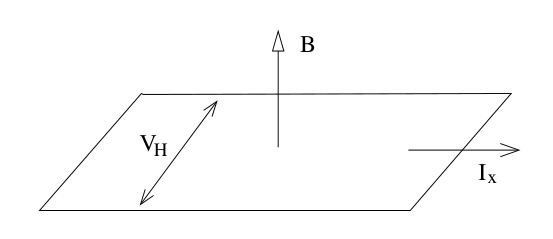
\includegraphics[scale=0.5]{figures/hall-effect.png}
	\caption[Scheme for the Quantum Hall Effect.]{Scheme for the Quantum Hall Effect. Taken from \cite{tong_lectures_2016}.}
\end{figure}
The electrons move in this plane with a circular motion due to the magnetic field $\vec{B}$ with a frequency,
\begin{equation}
	\omega_c=\frac{eB}{m}.
\end{equation}
This is called the \textit{ciclotron frequency. }
\subsubsection{Drude Model}
We can describe classically this effect using what we call the \textit{Drude Model.} Suppose we add an electric field $\vec{E}$  which will be responsible for accelerate the electrons in the absence of the magnetic field. We might consider the collisions that the electrons may have along the material with whatever can impede them. This was a first attempt to describe a conductor as if it was billiard balls. The equation of motion of this system is given by Newton's second law 
\begin{equation}
	m\frac{d\vec{v}}{dt}=-e\vec{E}-e\vec{v}\times\vec{B}-\frac{m\vec{v}}{\tau},
\end{equation}
where $\tau$ is the average time of collision of those particles.
We want the stationary solutions, that is, 
\begin{equation*}
	\frac{d\vec{v}}{dt}=0.
\end{equation*}
So we must solve the equation 
\begin{equation}
	e\vec{E}+e\vec{v}\times\vec{B}+\frac{m\vec{v}}{\tau}=0.
\end{equation}
Recalling that the current density is related to the velocity through the equation,
\begin{equation}
	\vec{J}=-ne\vec{v}.
\end{equation}
In matrix notation 
\begin{equation}
	\begin{pmatrix}1 & \omega_c\tau \\-\omega_c\tau & 1 \end{pmatrix}\vec{J}=\frac{e^2n\tau}{m}\vec{E}.
\end{equation}
And if we invert this relation, 
\begin{equation}\label{ohm law}
	\vec{J}=\sigma\vec{E}.
\end{equation}
This is \textit{Ohm’s Law}, which states how the current behaves in the presence of a electric field. We defined 
\begin{equation}
	\sigma=\begin{pmatrix}
		\sigma_{xx} & \sigma_{xy} \\
		\sigma_{yx} & \sigma_{yy} 
	\end{pmatrix},
\end{equation}
as the \textit{conductivity tensor}. This is something new that appears only in the presence of a magnetic field. Just as for the scalar case, the resistivity is the inverse of the conductivity, therefore 
\begin{equation}
	\rho =\sigma^{-1}.
\end{equation}
More explicitly,
\begin{equation}
	\rho =\frac{1}{\sigma_{DC}}\begin{pmatrix}1 & \omega_c\tau \\-\omega_c\tau & 1 \end{pmatrix}.
\end{equation}
The off-diagonal terms are responsible for the Hall effect. It can be shown that
\begin{equation}
	\rho_{xx}=\frac{m}{ne^2\tau},\quad \rho_{xy}=\frac{B}{ne},
\end{equation}
that graphically, is represented as
\begin{figure}[H]
	\centering
	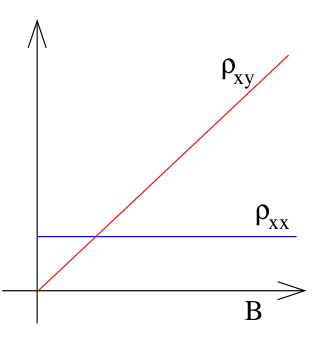
\includegraphics[scale=0.5]{figures/classical-hall-effect.png}
	\caption[Scheme for the Quantum Hall Effect.]{Expected resistivities for the classical Hall effect. Taken from \cite{tong_lectures_2016}.}
\end{figure}
\subsection{Integer Quantum Hall Effect}
The Quantum Hall Effect (QHE) was first discovered experimentally in 1980\cite{klitzing_new_1980}. It consists of the same scheme but now in regime where the magnetic field $\vec{B}$ is strong and temperature is low. The graph found for the resistivities was the one shown below. 
\begin{figure}[H]
	\centering
	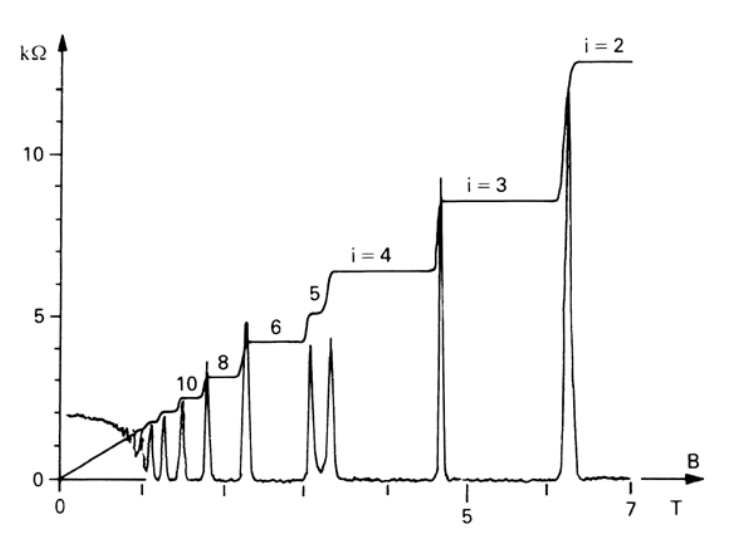
\includegraphics[scale=0.4]{figures/integer-qhe.png}
	\caption[Resistivities for the integer quantum Hall effect.]{Resistivities for the integer quantum Hall effect. Taken from \cite{tong_lectures_2016}.}
\end{figure}
This is completely different from that we expected classically. The plateux (that is, the areas in which the graph in plane) represent the transverse resistivity $\rho_{xy}$ and the spikes are the longitudinal resistivity $\rho_{xx}$. This is interesting because the resistivity over the plateux has the values
\begin{equation}
	\rho_{xy}=\frac{2\pi}{e^2}\frac{1}{\nu}, \;\nu\in\mathbb{Z},
\end{equation}
where the integer $\nu$ is called the \textit{filling fraction}. The center of these plateux occurs when the magnetic field assumes the values 
\begin{equation}
	B=\frac{2\pi n}{\nu e}=\frac{n}{\nu}\Phi_0. 
\end{equation}
In contrast, the values of $\rho_{xx}$ are zero most of the time, except when $\rho_{xy}$ changes its value. Then it spikes.  

What is fascinating about this effect is that a macroscopic quantity which is quantized, rather a microscopic one. Another aspect that is interesting, is that, in components, the conductivity is
\begin{equation}
	\sigma_{xx}=\frac{\rho_{xx}}{\rho_{xx}^2+\rho_{xy}^2},\quad \sigma_{xy}=\frac{-\rho_{xy}}{\rho_{xx}^2+\rho_{xy}^2}.
\end{equation}
If $\rho_{xy}=0$ we have 
\begin{equation}
	\sigma_{xx}=\frac{1}{\rho_{xx}}.
\end{equation}
Which  is a result that we are already familiar with, but in the case $\rho_{xx}=0$ with $\rho_{xy}\neq 0$ we have
\begin{equation}
	\sigma_{xx}=0.
\end{equation}
Apparently this case shows that our system is a perfect conductor and a perfect insulator simultaneously. But these are just names! What these expressions are really telling us is that, for $\sigma_{xx}=0$, no current is flowing in the longitudinal directions (just like an insulator) and $\rho_{xx}=0$ is telling us that no energy is being dissipated (just like a conductor). 

It is common to work with the QHE in terms of the conductivity,
\begin{equation}
	\sigma_{xy}=\frac{e^2}{2\pi}\nu.
\end{equation}
\subsection{Fractional Quantum Hall Effect}
The fractional QHE is even more exciting. The scheme is the same as the integer QHE but we now consider interactions between the electrons in the plane. What was found experimentally for the resistivities was
\begin{figure}[H]
	\centering
	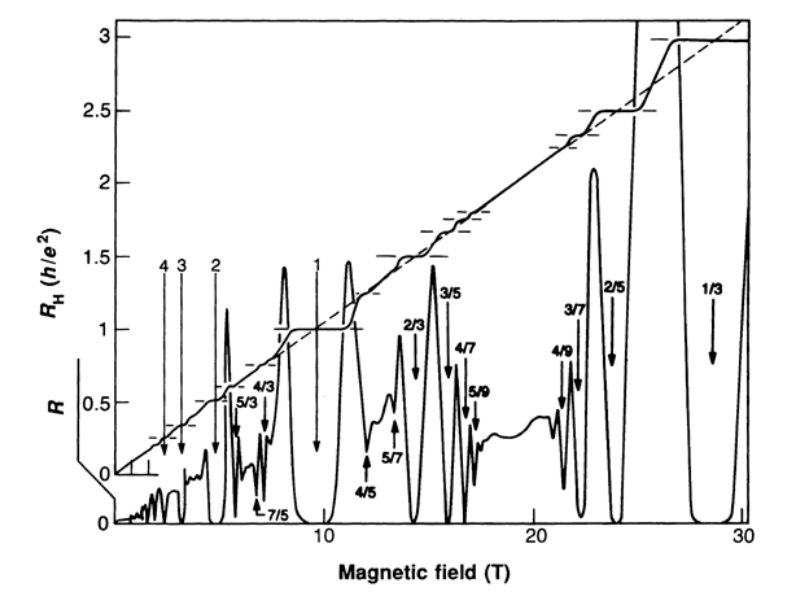
\includegraphics[scale=0.4]{figures/fractional-qhe.png}
	\caption[Resistivities for the fractional quantum Hall effect.]{Resistivities for the fractional quantum Hall effect. Taken from \cite{tong_lectures_2016}.}
\end{figure}
This shows that, in this case, the filling fractions may also assume \textit{fractional} values. And this is the reason for the name. We will dive deeper in the fractional QHE later when talking about its effective field theory. 
\section{Chern-Simons Theory}
One way we can describe the Quantum Hall Effect and obtain the results we have talked about is by relying on \textit{Chern Simons Theory}. The Chern Simons Theory is a gauge theory only conceivable in odd dimensions. In our case, we will study it in $D=3$\footnote{From now on, our convention is that $D$ means spacetime dimension and $d$ only spatial dimension.}.

It works this way because the new term that we add to the action, the \textit{Chern-Simons} term is, 
\begin{equation}
	S_{CS}=\frac{k}{4\pi}\int d^3x\;\epsilon^{\mu\nu\rho} A_\mu \partial _\nu A_\rho. 
\end{equation}
Note that indeed this theory will not work in 3+1 because of the Levi-Civita symbol. The indices do not match.  The constant $k$ is called the \textit{level} of the Chern-Simons term.

At first glance, the Chern-Simons action does not seem gauge invariant because it depends explicitly on the field $A_\mu$.  But upon a gauge transformation, 
\begin{equation*}
	S_{CS}\to S_{CS}+\frac{k}{4\pi}\int d^3x\; \partial_\mu(\omega\epsilon^{\mu\nu\rho}\partial_\nu A_\rho).
\end{equation*}
Thus, it changes by a total derivative. For some topologies, we can simply throw this term away. But in general, the boundary will have physical contributions. The Chern-Simons equations of motion are given by 
\begin{equation}
	F_{\mu\nu}=0.
\end{equation}
This shows that this theory has a trivial dynamics. This happens because the Chern-Simons term is a purely \textit{topological} term, in the sense that it does not depend on the spacetime metric. This can be seen explicitly if we write the action in terms of differential forms,
\begin{equation}
	S_{CS}=\int A\wedge dA. 
\end{equation}
and compare with the Maxwell action, 
\begin{equation}
	S_M=-\frac{1}{4e^2}\int F\wedge\star F. 
\end{equation}
To take the Hodge dual $\star F$ we need to use a metric, which has information about the geometry of the space. But the Chern-Simons, in contrast, does not involve any dual. Therefore it only depends on the topology of the manifold.

In (2+1) dimensions, the parity is defined as, 
\begin{equation*}
	x^0\to x^0,\;x^1\to -x^1,\; x^2\to x^2,
\end{equation*}
bcause if we were to define just like in 4 dimensions, that is  $\vec{x}\to -\vec{x}$,  since the matrix is 3-dimensional, it would have unit determinant and then would be a rotation. Therefore, we need to define that way. Note that the axis that we chose to be reflected is completely arbitrary and would work as well had we chose $x^2$ to be reflected. Upon those transformations, the gauge field transforms as,
\begin{equation*}
	A_0\to A_0,\;A_1\to-A_1,\;A_2\to A_2.
\end{equation*}
The integration measure $\int\;d^3x$  is invariant under parity because even if $x_1\to -x_1$, the integration limits also change. But the integrand is not invariant, that is 
\begin{equation*}
	\epsilon^{\mu\nu\rho}A_\mu\partial_\nu A_\rho\to-\epsilon^{\mu\nu\rho}A_\mu\partial_\nu A_\rho.
\end{equation*}
Thus the Chern-Simons term can only arise in theories that break parity. 

We know that the conserved current couples with the gauge field as
\begin{equation*}
	S=\int d^3x\;J^\mu A_\mu. 
\end{equation*}
This shows that 
\begin{equation*}
	\frac{\delta S}{\delta A_\mu}=J^{\mu}.
\end{equation*}
Which implies,
\begin{equation}
	J_i=-\frac{k}{2\pi}\epsilon_{ij}E_j.
\end{equation}
From (\ref{ohm law}),
\begin{equation*}
	\vec{J}=\sigma\vec{E}.
\end{equation*}
Hence
\begin{equation*}
	\sigma_{xy}=\frac{k}{2\pi}.
\end{equation*}
This coincides with the Hall conductivity if we identify
\begin{equation}\label{ch level quantized}
	k=e^2\nu.
\end{equation}
But there is nothing that tell us that $\nu$ should be quantized. We will see how this works shortly.
\subsection{Topological mass generation}
Before we talk about the quantization of the Chern-Simons level, let us study the effect of adding Chern-Simons term along with other gauge theories. Take the Maxwell-Chern-Simons Lagrangian
\begin{equation}
	\mathcal{L}_{\text{{MCS}}}=-\frac{1}{4e^2}F_{\mu\nu}F^{\mu\nu}+\frac{k}{4\pi}\epsilon^{\mu\nu\rho}A_{\mu}\partial_{\nu}A_{\rho}.
\end{equation}
The equations of motion are,
\begin{equation}
	\partial_{\mu}F^{\mu\nu}+\frac{ke^2}{4\pi}\epsilon^{\nu\alpha\beta}F_{\alpha\beta}=0.
\end{equation}
Introducing the dual field $\tilde{F}^\mu$, 
\begin{equation}
	\tilde{F^{\mu}}=\frac{1}{2}\epsilon^{\mu\nu\rho}F_{\nu\rho}\Rightarrow\tilde{F_{\mu}}=\frac{1}{2}\epsilon_{\mu\alpha\beta}F^{\alpha\beta},
\end{equation}
we can invert the relation by multiplying by a Levi-Civita both sides, which gives
\begin{equation}
	F^{\sigma\rho}=\epsilon^{\mu\sigma\rho}\tilde{F_{\mu}.}
\end{equation}
Then we get
\begin{equation*}
	\epsilon^{\alpha\mu\nu}\partial_{\mu}\tilde{F_{\alpha}}+\frac{ke^2}{2\pi}\tilde{F^{\nu}}=0.
\end{equation*}
This can be re-written as 
\begin{equation}
	\left(\partial_{\mu}\partial^{\mu}+\left(\frac{ke}{2\pi}\right)^{2}\right)\tilde{F^{\sigma}}=0.
\end{equation}
This is the equation of motion for a field with mass $m=\frac{ke}{4\pi}$.  

Another way to see this is trough the propagator. Recall from LSZ reduction formula that in order to compute the $S$-matrix elements, we need to evaluate the following expression, 
\begin{equation}\label{lsz formula}
	\begin{split}
		\langle p_1\dots p_n | S | q_1\dots q_n\rangle = \prod_{r=1}^{n}\lim_{p^2_r\to m^2_r}(p_r^2-m_r^2)J_{i_{r}}(p_r)\prod_{s=1}^{m}\lim_{p^2_s\to m^2_s}(q_s^2-m_s^2)J_{i_{s}}(p_s)\\\times G_{i_{1}\dots j_{m}}(p_1,\dots,p_n,-q_1,\dots,-q_m),
	\end{split}
\end{equation}
where $ G_{i_{1}\dots j_{m}}(p_1,\dots,p_n,q_1,\dots,q_m)$ is the propagator. Since propagators are often the form $\frac{1}{p^2-m^2}$, the poles are interpreted as the masses of the field.  
Rewriting the Lagrangian as 
\begin{equation*}
	\mathcal{L_{\text{MCS}}}=A_{\mu}\left[\frac{1}{2e^2}g^{\mu\nu}\Box-\frac{k}{4\pi}\epsilon^{\mu\rho\nu}\partial_{\rho}-\frac{1}{2e^2}\left(\frac{1}{\xi}-1\right)\partial^{\mu}\partial^{\nu}\right]A_{v},
\end{equation*}
with a gauging fixing term $-\frac{1}{2\xi e^2 }(\partial_\mu A^\mu)^2$, we identify the term between brackets as the inverse of the propagator, 
\begin{equation}
	(\Delta^{-1})^{\mu\nu}=\frac{1}{2e^2}g^{\mu\nu}\Box-\frac{k}{4\pi}\epsilon^{\mu\rho\nu}\partial_{\rho}-\frac{1}{2e^2}\left(\frac{1}{\xi}-1\right)\partial^{\mu}\partial^{\nu}.
\end{equation}
In the momentum space this is written as 
\begin{equation}
	(\Delta^{-1}(p))^{\mu\nu}=\frac{1}{2}g^{\mu\nu}p^2+\frac{ik}{4\pi}\epsilon^{\mu\nu\rho}p_\rho+\frac{1}{2}\left(1-\frac{1}{\xi}\right)p^\mu p^\nu.
\end{equation}
To compute the propagator, first we introduce the following operators,
\begin{equation}
	\omega^{\mu\nu}\equiv\frac{p^\mu p^\nu}{p^2},\;S^{\mu\nu}\equiv i\epsilon^{\mu\nu\rho}p_\rho,\;\theta^{\mu\nu}=g^{\mu\nu}-\omega^{\mu\nu}.
\end{equation} 
These form a closed algebra,
\begin{equation}
	\omega^2=0,\;\;\omega\cdot\theta=0,\;\;\\\theta^2=0,\;\;\omega\cdot S=0,\;\;\\S^2=-p^2\cdot\theta,\;\theta\cdot S=S.
\end{equation}
The propagator in this basis should have the form,
\begin{equation}
	\Delta_{\mu\nu}(p)=A\omega_{\mu\nu}+B\theta_{\mu\nu}+CS_{\mu\nu}, 
\end{equation}
with $A,B,C$ complex numbers. Thus, we need to solve the equation 
\begin{equation}
	\Delta_{\mu\alpha}(\Delta^{\alpha\nu})^{-1}=\delta_\mu^{\;\;\nu},
\end{equation}
for $A,B$ and $C$. The propagator then will be given by 
\begin{equation}
	\Delta_{\mu\nu}=\left(\frac{p^2g_{\mu\nu}-p_\mu p_\nu-\frac{ike^2}{2\pi}\epsilon_{\mu\nu\rho}p^\rho}{p^2(p^2-(\frac{ke^2}{2\pi})^2)}+\xi\frac{p_\mu p_\nu}{p^4}\right).
\end{equation}
Thus, we obtain again that the mass of the gauge field is $\left(\frac{ke}{2\pi}\right)^2.$ Note that it seems that we also have a pole at $p^2=0$, but that pole is actually ``fake''. This can be seen from Eq.(\ref{lsz formula}). The conserved currents can be written in a basis that depends on the momentum $p$ and the polarization vectors $\epsilon$. Therefore the products of the form $J \Delta J$ will give zero or cancel the $p^2$ on the denominator. The only case where this does not follow straightforward is the term with the Levi-Civita symbol. In this case, the conservation law $p_\mu j^\mu=0$ will impose a constraint in the components, which will cancel each other. 


This shows that the coupling with the Chern-Simons term works as some kind of “Higgs mechanism”, giving a mass to the gauge field. We call this a “topological mass'' due to the nature of the Chern-Simons theory.  

We may have the Higgs mechanism as well. This is the Maxwell-Chern-Simons-Higgs Lagrangian
\begin{equation}
	\mathcal{L_{\text{MCSH}}}=-\frac{1}{4}F_{\mu\nu}F^{\mu\nu}+\frac{k}{4\pi}\epsilon^{\mu\nu\rho}A_{\mu}\partial_{\nu}A_{\rho}+(\mathcal{D_{\mu}}\phi)^{*}\mathcal{D}^{\mu}\phi-V(|\phi|),
\end{equation}
where $V(|\phi|)$ is some symmetry-breaking potential with non-trivial minimum $\langle \phi\rangle =v$. As we did in Chapter \ref{chap:ssb}, we may parametrize the field as $\phi = \rho e^{i\varphi}$, leading to
\begin{equation}
	\begin{split}
		\mathcal{L}_{MCSH} &= -\frac{1}{4}F_{\mu\nu}F^{\mu\nu} +\frac{k}{4\pi} \epsilon^{\mu\nu\rho}A_\mu\partial_{\nu}A_\rho + \partial_{\mu}\rho\partial^\mu\rho + \rho^2(eA_\mu+\partial_\mu\varphi)^2 - V(\rho).
	\end{split}
\end{equation}
Expanding the field around the minima as $\rho = \tilde{\rho} + v$, we get 
\begin{equation}
	\begin{split}
		\mathcal{L} &=-\frac{1}{4}F_{\mu\nu}F^{\mu\nu} +\frac{k}{4\pi} \epsilon^{\mu\nu\rho}A_\mu\partial_{\nu}A_\rho + \partial_{\mu}\tilde{\rho}\partial^\mu\tilde{\rho} + v^2(eA_\mu+\partial_\mu\varphi)^2 - V(|\phi|) \\& + \text{cubic terms} + \text{quartic terms.}
	\end{split}
\end{equation}
To compute the propagator for $A_\mu$, we only need the quadractic terms o involving $A_\mu$. We can choose a gauge fixing term that kills the field $\varphi$, 
\begin{equation}
	A_\mu \to - A_\mu + \frac{1}{e^2}\partial_\mu\varphi.
\end{equation}
If we use the same algorithm that we have used to the Maxwell-Chern-Simons Lagrangian, the propagator for the gauge field will be 
\begin{equation}
	\begin{split}
		\Delta_{\mu\nu}&=\frac{e^{2}(p^{2}-m_{H}^{2})}{(p^{2}-m_{+}^{2})(p^{2}-m_{-}^{2})}\left[g_{\mu\nu}-\frac{p_{\mu}p_{\nu}}{(p^{2}-\xi m_{H}^{2})}-\frac{i}{2\pi}\frac{ke^{2}\epsilon_{\mu\nu\rho}p^{\rho}}{(p^{2}-m_{H}^{2})}\right]\\&+e^{2}\xi\frac{p_{\mu}p_{\nu}(p^{2}-(\frac{ke^2}{2\pi})^2-m_{H}^{2})}{(p^{2}-m_{+}^{2})(p^{2}-m_{-}^{2})(p^{2}-\xi m_{H}^{2})},
	\end{split}
\end{equation}
where $m_{H}^{2}=2e^{2}v^{2}$  is the Higgs mass i.e, the mass generated by the Higgs mechanism and 
\begin{equation}
	m_{\pm}^{2}=m_{H}^{2}+\frac{(ke^{2})^{2}}{8\pi^2}\pm\frac{ke^{2}}{4\pi}\sqrt{\left(\frac{ke^2}{2\pi}\right)^2+4m_{H}^{2}},
\end{equation}
are the topological masses of the gauge field. So what we have here is the following. In the unbroken vacumm, the complex scalar field has two massive degress of freedom and the gauge field has one massive degree of freedom arising from the Chern-Simons term. In the broken vacuum, one component of the scalar field combines with the longitudinal degree of freedom of the gauge field, resulting in one massive degree of freedom for the scalar field and two massive degrees of freedom from the gauge field.

Therefore, the photon has acquired a topological mass due to the Chern-Simons term and a Higgs mass due to the Higgs mechanism. Note that we can also work with a Chern-Simons-Higgs Lagrangian only if we take the limit
\begin{equation}
	e^2\to\infty,\quad k=\text{fixed. }
\end{equation}
In this case, the Lagrangian becomes
\begin{equation}
	\mathcal{L_{\text{CSH}}}=\frac{k}{4\pi}\epsilon^{\mu\nu\rho}A_{\mu}\partial_{v}A_{\rho}+(\mathcal{D_{\mu}\phi})^{*}\mathcal{D^{\mu}}\phi-V(|\phi|).
\end{equation}
To compute the degrees of freedom we can take this limit in the Maxwell-Chern-Simons-Higgs Propagator, leading to 
\begin{equation}
	\Delta_{\mu\nu}=\frac{1}{p^{2}-\left(\frac{4\pi v^{2}}{k}\right)^{2}}\left[\frac{4\pi v^{2}}{k}g_{\mu\nu}-\frac{p_{\mu}p_{\nu}}{2v^{2}}+\frac{i}{k}\epsilon_{\mu\nu\rho}p^{\rho}\right],
\end{equation}
in which we identify a mass pole at $p^{2}=\left(\frac{4\pi v^{2}}{k}\right)^{2}$.  Thus, in the unbroken vacuum the gauge field is non-propagating and the scalar field has two massive degrees of freedom. In the broken vacuum, one of the components of the scalar field combines with the longitudinal component of the gauge field giving a mass $\frac{4\pi v^{2}}{k}$ to it. Note that we can rewrite $m_{\pm}$  as 
\begin{equation}
	m_{\pm}=\frac{ke^{2}}{4\pi}\left(\sqrt{1+\frac{32\pi^{2}v^2}{(ke^2)^{2}}}\pm1\right).
\end{equation}
Taking the limit $e^2\to\infty$, 
\begin{equation}
	m_{\pm}\sim\frac{ke^{2}}{4\pi}\left(1+\frac{16\pi^2v^{2}}{(ke^2)^{2}}\pm1\right)=\frac{ke^{2}}{4\pi}+\frac{4v^{2}}{k\pi}\pm\frac{ke^{2}}{4\pi}.
\end{equation}
Thus we have that $m_{+}\to\infty$ and $m_{-}\to2v^{2}/2,$ highlighting that indeed the gauge field has only one massive degree of freedom. 
\subsection{Quantization of the Chern-Simons Level}
We have seen above that the Chern-Simons theory described the correct expression for the Hall conductivity but there was nothing telling us that the filling factor $\nu$ should be quantized. We now proceed to show this. 

The quantization of the Chern-Simons level is not easy to perform given, the fact that the Chern-Simons theory is a constrained theory and therefore it should be quantized using Dirac brackets\cite{Dirac_1950}. Nonetheless, we can obtain the results for the QHE without having to enter this heavy mathematical formalism. In order to do this, we must first perform a very common technique in field theory that is called a \textit{Wick rotation,} which enable us to connect statistical mechanics with the path integral formalism. 

For simplicity, we will do this for a system of a single particle in a potential $V(q)$. The partition function for this system is 
\begin{equation}
	Z[\beta]=\Tr e^{-\beta H},
\end{equation}
where $\beta=1/T$ and $H$ is the Hamiltonian. Recall from the path integral formalism that the a probability amplitude is given by\footnote{For the reader that is unfamiliar with the path integral formalism, a nice discussion can be found in \cite{nakahara_geometry_2003}.} 
\begin{equation}
	\langle q_f|e^{-iHt}|q_i \rangle=\int_{q(0)=q_i}^{q(t)=q_f} \mathcal{D}q\;e^{iS}.
\end{equation}
We note that these two objects have a similar form. To get rid of the factor of $i$, we can change the variable $t$ to 
\begin{equation}
	\tau = it,
\end{equation}
this is what we call a Wick rotation. Hence, the action of the particle will change as
\begin{equation}
	S=\int_0^{-i\tau} \frac{dt}{d\tau'}d\tau' \;L(\dot{q},q)=-i\int_0^{-i\tau}d\tau'\left[-\frac{m}{2}\left(\frac{dq}{d\tau}\right)^2-V(q)\right]\equiv -S_E,
\end{equation}
where $S_E$ is called a \textit{Euclidean action}. We will use this notation only on this section to make the distinction clear, but in what follows we will no longer use it. It can seen that the Euclidean action is being used when there are no factors of $i$ accompanying the action. 

Now, to get the $\beta$ factor we want, we can say that the particle propagates during an Euclidean time $\tau=\beta$. Then the amplitude becomes 
\begin{equation*}
	\langle q_f|e^{-H\beta}|q_i \rangle=\int_{q(0)=q_i}^{q(\beta)=q_f} \mathcal{D}q\;e^{-S_E}.
\end{equation*}
To obtain the trace, we must recall that the trace is a sum over the \textit{same} states. In this amplitude, we have different states $|q_i\rangle$ and $|q_f\rangle$. Then, we must demand that the particle return to its initial position. We do this by making the time periodic,
\begin{equation*}
	\tau \sim \tau +\beta. 
\end{equation*}
Therefore, the partition function becomes 
\begin{equation}\label{partition function}
	Z[\beta]=\int\mathcal{D}q\; e^{-S},
\end{equation}
where we have dropped the $S_E$ notation. Note that this mapping implies that our time, the Euclidean time, has become a $S^1$. This must be considered in our further calculations. We can now proceed to the quantization. 

For simplicity, consider our space to be a $S^2$. Therefore our spacetime is a manifold $\mathcal{M}=S^1\times S^2$. There is another thing that simplifies our calculations. Suppose we have a magnetic monopole in the origin with flux
\begin{equation}
	\int_{S^2} d\vec{a}\cdot \vec{B}=g,
\end{equation} 
where $g$ is quantized via the Dirac condition, from Chapter 2, 
\begin{equation}
	eg=2\pi n,n\in\mathbb{Z}.
\end{equation}
This may seem biased, since magnetic monopoles do not exists  (yet). But what we are assuming is that, this should hold even in the presence of monopoles. A different and more mathematical approach, using wavefunctionals, can be found in \cite{dunne_aspects_1999, dunne_topological_1990,girvin_quantum_1999}. 

The Dirac condition in terms the field strenght is (considering $g=1$)
\begin{equation}
	\int_{S^2}F_{12}=\frac{2\pi}{e}.
\end{equation}
The gauge transformation is, as usual 
\begin{equation*}
	A_{\mu}\to A_{\mu}+\partial_{\mu}\Lambda. 
\end{equation*}
Because of the periodicity of our time, we can choose a gauge that is periodic in time as well, 
\begin{equation}
	\Lambda=\frac{2\pi\tau}{e\beta}.
\end{equation}
That way, the gauge transformation for $A_0$ is given by 
\begin{equation}
	A_0'=A_0+\frac{2\pi}{e\beta}.
\end{equation}
These are called \textit{large gauge transformations} and are related to gauge transformations that are periodic and have a non-trivial winding. But as we have seen, under gauge transformations, the action changes as 
\begin{equation}
	\begin{split}
		S_{CS}&\to S_{CS}+\frac{k}{4\pi}\int d^3x\; \partial_\mu(\omega\epsilon^{\mu\nu\rho}\partial_\nu A_\rho)\\ &= S_{CS}+\frac{2\pi k}{e^2},
	\end{split}
\end{equation}
which highlights the fact that the action is not invariant under gauge transformations.  However, in QFT, the partition function is a more fundamental object than the action. Therefore, it is no problem that the action changes under large gauge transformations, as long as the partition functions does not change. From (\ref{partition function}) we have
\begin{equation}
	Z[A_\mu]=e^{iS[A_\mu]}.
\end{equation}
Thus, we see that it is invariant if
\begin{equation}
	\frac{k}{e^2}\in\mathbb{Z}.
\end{equation}
But from eq.(\ref{ch level quantized}),
\begin{equation*}
	k=e^2\nu.
\end{equation*}
Therefore, $\nu$ is indeed an integer. So we have successfully shown that the Chern-Simons level is quantized and that it describes that correct conductivities of the integer QHE. We now proceed to describe the fractional QHE.  
\subsection{Effective field theory for the fractional QHE}
The fractional quantum Hall effect can be described usign Chern-Simons theory as well. The novelty is that now we will take into account the interaction between the electrons. 

We start by introducing an emergent $U(1)$ gauge field $a_\mu$, associated to the collective motion of the underlying electrons. This is different from the gauge field $A_\mu$ from Maxwell theory. The simplest term that we can add to the action involving this field is the Chern-Simons term,
\begin{equation}
	S_{CS}=\frac{k}{4\pi}\int d^3x\;\epsilon^{\mu\nu\rho}a_\mu \partial_\nu a_\rho. 
\end{equation}
Despite the fact that the field $a_\mu$ is not the Maxwell field, it follows the same properties that we have seen before. It  has its own dynamics given by 
\begin{equation}
	S[a_\mu]=-\frac{1}{4}\int d^3x\;f_{\mu\nu}f^{\mu\nu},
\end{equation}
and it works as a topological mass generator as well. 

The states that describe the fractional QHE are the Laughlin states \cite{PhysRevLett.50.1395}. We now will write down an action that is able to describe those states and therefore reproduce the expected values for the Hall conductivity. First we need a coupling between the fields $A_\mu$ and $a_\mu$. In general the coupling involving gauge fields is trough a conserved current. Luckily, we have a perfect conserved current to couple with. It is 
\begin{equation}\label{electron current}
	j^{\mu}=\frac{1}{2\pi}\epsilon^{\mu\nu\rho}\partial_\nu a_\rho,
\end{equation}
where its conservation result from the contraction of the two derivatives with the Levi-Civita symbol. We can interpret this as if the magnetic flux of $a_\mu$ is the electric charge that couples with $A_\mu$. This magnetic flux also follows the Dirac quantization condition 
\begin{equation}
	\frac{1}{2\pi}\int_{S^2}f_{12}=\frac{\hbar}{e}.
\end{equation}
The normalization ensures that the minimum charge allowed is $\int J^0=e$, as it should be. The effective action is then 
\begin{equation}
	S_{eff}[A;a]=\int d^3x\;\frac{1}{2\pi}\epsilon^{\mu\nu\rho}A_\mu\partial_\nu a_\rho-\frac{m}{4\pi}\epsilon^{\mu\nu\rho}a_\mu\partial_\nu a_\rho+...\;.
\end{equation}
The first term is the coupling and the second is the Chern-Simons term for $a_\mu$. We have used $m$ instead of $k$ because it is a different term (although it has the same functional form), from the Chern-Simons term for integer QHE. The other terms that may arise vanish at large distances and therefore we do not need them to our conclusions. There could be also a Chern-Simons term for the $A_\mu$ field, but this is just the term we had on the integer QHE and we would just obtain again the conclusion that the level $k$ should be quantized. For the same reasons that $k$ is quantized, $m$ is also quantized. Computing the equation of motion for $a_\mu$, we have  
\begin{equation}
	f_{\mu\nu}=\frac{1}{m}F_{\mu\nu}.
\end{equation}
This has the solution, 
\begin{equation}
	a_\mu=\frac{1}{m}A_{\mu}.  
\end{equation}
Substituting back in the action, 
\begin{equation}
	S_{eff}[A]=\int d^3x\;\frac{1}{4\pi m}\epsilon^{\mu\nu\rho}A_{\mu}\partial_\nu A_\rho. 
\end{equation}
This term is again a Chern-Simons term but with level $1/m$. Thus, doing the same process, we will obtain the Hall conductivity to be 
\begin{equation}
	\sigma_{xy}=\frac{e^2}{2\pi}\frac{1}{m}.
\end{equation}
This shows that indeed, the Hall conductivity in the fractional QHE may assume fractional values as well, with the filling factor being $\nu=1/m$. There are some subtleties about this derivation because the effective action has some troubles when integrating over a $S^2$. Moreover, the fields are constrained by the Dirac quantization condition, and the equation of motion is not satisfied when both have a single unit of flux. But these subtleties lies in the manifold structure of our space and it has to do with the choice of charts, something that we will not dive into.
\subsection{Charged excitations}
In the Chern-Simons theory we may have two types of charged excitations. These are the \textit{quasi-holes} or \textit{quasi-particles}. In what follows, we will derive a remarkable property of these excitations, which are verified in the QHE. We will not make any distinction in this section and every excitation will be called a quasi-particle. 

Take Chern-Simons action and add a term for the current of the quasi-particles $\tilde{j}^\mu$, 
\begin{equation}
	S[a;A]=\int d^3x\frac{1}{2\pi}\epsilon^{\mu\nu\rho}A_\mu\partial_\nu a_\rho-\frac{k}{4\pi}\epsilon^{\mu\nu\rho}a_\mu\partial_\nu a_\rho+a_\mu \tilde{j}^\mu +\dots.
\end{equation}
Since $A_\mu$ is a background field, we can set it to zero. The equations of motion then will be given by 
\begin{equation}
	\frac{1}{2\pi}f_{\mu\nu}=\frac{1}{k}\epsilon_{\mu\nu\rho}\tilde{j}^{\rho}.
\end{equation}
The simplest charge we can consider is a static charge at the origin. These will have the components, 
\begin{equation}
	\tilde{j}^1=\tilde{j}^2=0,\;\tilde{j}^0=e\delta^2(x).
\end{equation}
The choice for the charge of these particles is due to the Dirac quantization. Therefore the equations of motion become, 
\begin{equation}
	\frac{1}{2\pi}f_{12}=\frac{e}{k}\delta^2(x).
\end{equation}
This shows that the role of the Chern-Simons term is to attach a magnetic flux $e/k$ to each particle of charge e. 


From Eq.(\ref{electron current}), we note that the charge of these particles is the zeroth component, thus 
\begin{equation}
	j^0=\frac{1}{2\pi}\epsilon^{ij}\partial_i a_j= \frac{1}{2\pi}f_{12}=\frac{e}{k}\delta^2(x).
\end{equation}
This shows that the electron charge in Chern-Simons theory is fractional. Therefore, the charged excitations in Chern-Simosn theory are charges with a fraction of the electron charge with a magnetic flux atteched to them. Below, we show schematically the quasi-particles in Chern-Simons theory.
\begin{figure}[H]
	\centering
	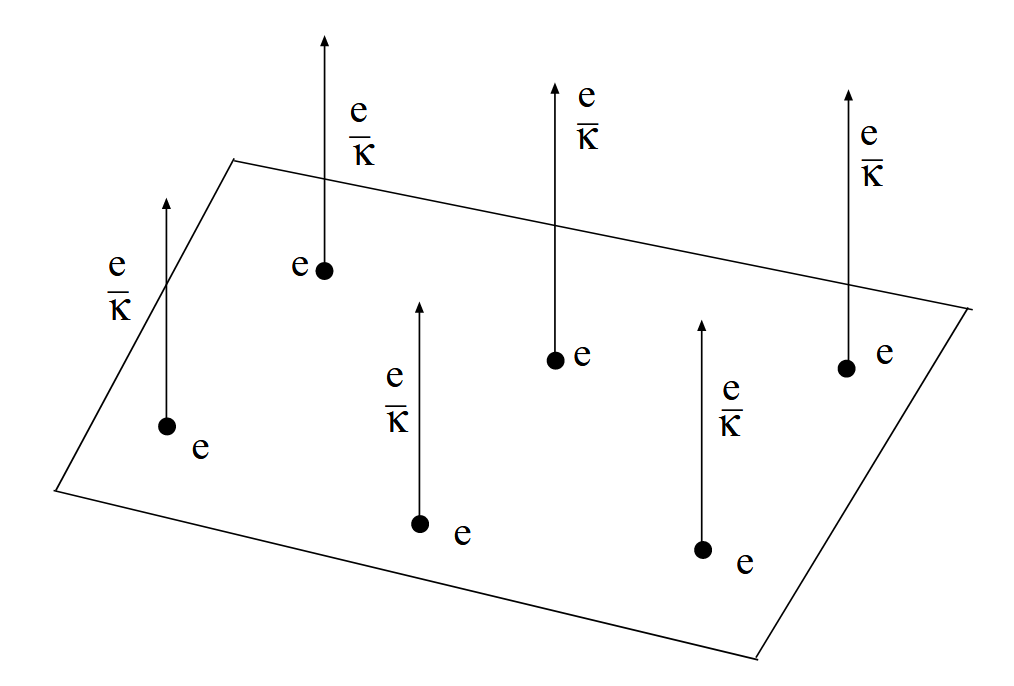
\includegraphics[width=0.7\linewidth]{figures/quasi-particles-cs}
	\caption[Quasi-particles in Chern-Simons theory]{Quasi-particles in Chern-Simons theory. Taken from \cite{dunne_aspects_1999}.}
	\label{fig:quasi-particles-cs}
\end{figure}
\noindent Consider now a more general current, 
\begin{equation}
	j^0(\vec{x},t)=e\sum_{a=1}^{N}\delta^2(\vec{x}-\vec{x}_a(t)),\; \vec{j}(\vec{x},t)=e\sum_{a=1}^{N}\dot{\vec{x}}_a(t)\delta^2(\vec{x}-\vec{x}_a(t)).
\end{equation}
Imposing $\partial_i a_i=0,$ we conclude that,
\begin{equation}
	a_i = \epsilon_{ijk}\partial_j \chi_k. 
\end{equation}
Solving the two-dimensional Green's function in the gauge $a_0=0$ we find,
\begin{equation}
	a_i(\vec{x},t)=\frac{e}{k}\sum_{a=1}^N\epsilon^{ij}\frac{x^j-x^j_a}{|\vec{x}-\vec{x}_a(t)|^2}.
\end{equation}
Using the identity, 
\begin{equation}
	\partial_i\text{arg}(\vec{x})=-\epsilon_{ij}\frac{x^j}{|\vec{x}|^2}, \quad \text{arg}(\vec{x})=-\arctan\left(\frac{y}{x}\right).
\end{equation}
We obtain,
\begin{equation}
	a_i(\vec{x})=\frac{e}{k}\sum_a\partial_i\arg(\vec{x}-\vec{x}_a).
\end{equation}
One can think that this field is a pure gauge and then we could transform this field to zero by chosing 
\begin{equation}
	a_i'=a_i+\partial_i\Lambda,\quad \Lambda=-\frac{e}{k}\sum_a\arg(\vec{x}-\vec{x}_a).
\end{equation}
But under gauge transformations, the wavefunction of the electrons would change as 
\begin{equation}
	\psi\to e^{ie\Lambda}\psi=\exp\left(-\frac{e^2}{k}\sum_a\arg(\vec{x}-\vec{x_a})\right)\psi.
\end{equation}
Thus, we see that this wavefunction is not single valued and therefore the phase cannot be ignored.

In fact, it is this non-trivial reminiscent phase that gives a very interesting aspect of this theory. Consider that we move a particle around another. Since these particles have magnetic flux attached to them, upon returning to the same point, they will acquire an Aharanov-Boohm phase $\exp\left(ie\oint_C\vec{A}\cdot d\vec{x}\right)$. Hence 
\begin{equation}
	\exp\left(\frac{i\hbar}{k}\sum_{a=1}^{N}\oint\partial_i\arg(\vec{x}-\vec{x}_a)dx^i\right)=e^{\frac{2\pi i}{k}}
\end{equation}
But considering an exchange of the two particles is equivalent to perform half of a turn and then a translation. This will give the phase $e^{\frac{\pi i}{k}}$. Therefore, we conclude that the exchanging phase is fractional. The braiding is a way of measuring the statistics of two particles. Since this is not an integer (which would correspond to a boson) nor half-integer (which would correspond to a fermion) we call these particles with unusual statistics \textit{anyons.}

\bibliography{refs.bib}
\bibliographystyle{ieeetr}

\end{document}
